\section{Implementation}
\label{sec:implementation}

Using our operationalization of the five star model of data sharing
 in section \ref{sec:operationalization} we created
 a web observatory for linked open data,
 called \obs.\footnote{Code and results available at
   \url{https://github.com/wouterbeek/LODObs}}

\obs uses an automated script in order to look for
 data on the Web.
The script must be given a set of locations where Web data
 is likely to be found.
For this we use CKAN API.\footnote{\url{http://docs.ckan.org}}
CKAN is an open-source data portal platform
 that allows datasets that are published on the Web to be catalogued.
There are various catalogues available,
 including the governmental initiatives towards data sharing
 of the UK and the USA.

\obs gives a tabular overview of the results of
 processing the various resources, see Figure \ref{fig:lod_observer}.
\obs provides more detailed information than we are able to give
 in our results section (i.e. section \ref{sec:results});
 e.g. it shows the specific error messages encountered
 and the syntax error that occur while reading a serialization format.

\begin{figure*}[th!]
  \label{fig:lod_observer}
  \centering
  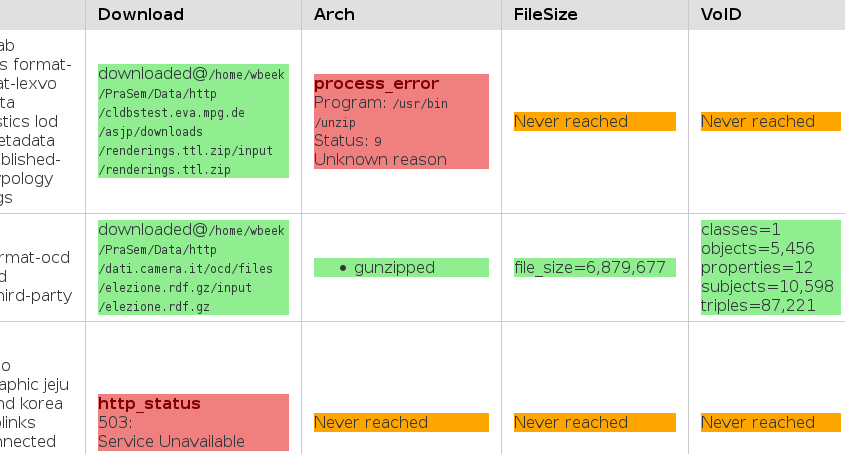
\includegraphics[width=0.85\textwidth]{./img/table}
  \caption{
    A part of the table that is generated by \obs.
    Each row in the table displays the results of retrieving a single
     resource from Datahub.
    Each column in the table corresponds to a specific action
     that is performed for a specific resource.
    The picture shows the results of executing the following four actions
     for three resources:
     (1) downloading the resource,
     (2) unarchiving it,
     (3) determining the file size, and
     (4) counting some basic VoID statistics \cite{Void2011}.
  }
\end{figure*}

\subsubsection*{Locating resources}

CKAN uses URLs as universal locators for resources.
URLs are URIs that identify a resource via a representation of
 its primary access mechanism or scheme (e.g. HTTP)
 and its network location (e.g. \texttt{www.datahub.io})
 that can be accessed using standardized operations
 defined for that scheme. \cite{Rfc3305}

The datasets that are catalogued by CKAN provide
 a starting point for an automated agent to search for data on the Web,
 since all data registrations can be queried using an API.
Since datasets have to be explicitly registered at a CKAN catalogue,
 this ensures that they are purposefully published
 as machine-processable data,
 thereby following our definition of a `resource'
 (see section \ref{sec:operationalization})
Each CKAN resource has a URL property field,
 which allows an automated agent to find a URL string for each resource.

\subsubsection*{Connecting to disseminating host}

When using the URL string to locate a resource we find that
 not all URL strings parse according to the grammar
 in the URL specification \cite{Rfc3986},
 and some URLs that are grammatically correct contain a scheme
 that is not registered with
 the Internet Assigned Numbers Authority
 (IANA).\footnote{\url{http://www.iana.org/assignments/uri-schemes/uri-schemes.xhtml}}
%\footnote{
%  The number of resources for which the URL string parses correctly
%  can be increased by trimming leading and trailing whitespace (US-ASCII 32)
%  and by prepending the string with a commonly occurring scheme descriptor
%  (e.g., \texttt{http://}) in case the grammar cannot detect a scheme.
%}

Culprits:
\begin{itemize}[noitemsep,nolistsep]
  \item The URL string does not parse according to the RFC grammar.
  \item The parsed URL string does not contain an IANA-registered scheme.
\end{itemize}

For URLs that are grammatically correct an automated agent is able to
 verify whether there exists a host authority at the location
 denoted by the URL.
As with the Web of Documents, this is not always the case,
 resulting in a ``host not found exception''.
Once a host authority is found, it has to accept a connection
 with the automated agent.
Only when a connection is established can the agent send its request
 to the authority.
The agent and authority both have to maintain the connection
 for the duration of the subsequent request/response-interaction.

Culprits:
\begin{itemize}[noitemsep,nolistsep]
\item The host that is denoted by the URL's authority string cannot be found.
\item The connection was refused by the host.
\item The connection was neither refused nor accepted by the host.
\item The connection was established, but was broken off
      during subsequent communication.
\item The host was redirecting the connecting agent indefinitely.
\end{itemize}

\subsubsection*{Retrieving resource from host}

Once a reliable connection between agent and host is established
 for the duration of a communicative interaction,
 the agent is able to send a request in one of
 the standardized Internet communication protocols.
Specifically, \obs supports communications via FTP and HTTP(S).

Various things can go wrong in both formulating the request and
 in replying to it.
This results in various status codes that denote different problems
 that cause the communication to be ineffective.

\subsubsection*{Open license}

Many CKAN registered resources have a license property.
The licenses are similar to those defined by the Open Data Commons,
 but some mismatches occur.
In the Datahub CKAN repository, 33 licenses are used,
 18 of which are underdefined (i.e., with no semantic description),
 impacting 5\% of the resources.
We have added manual mappings from the CKAN licenses onto
 the repository of Open Data Commons license descriptions.
%This results in added descriptions for 14 underdefined licenses,
% additional properties for 4 licenses that were already partially defined,
% and leaves only 2 underdefined licenses that have been equated to
% `license' \texttt{ckan:None} using \texttt{owl:sameAs} statements.

Culprits:
\begin{itemize}[noitemsep,nolistsep]
\item Has no license string.
\item Has a license string that cannot be mapped to
       a license that occurs in
       the Open Data Commons license description set.
\item Has a recognized license that is not open.
\end{itemize}

\subsubsection*{Structured \& non-propetary}
\label{sec:implementation_mime}

In order to implement the structuredness requirement,
 we have manually classified the MIME types that occur in the CKAN catalogue
 into `structured' and `unstructured' ones.
This goes against our interpretation of structuredness as
 a gradient property, but the partial order constituted by the relation
 ``supports at least the same set of relational operators''
 cannot be easily established in an automated way,
 as this would require a model of query operators
 and a description of MIME types in terms of the operators that are
 supported by those content types.

We list the 4 ways in which we can check for a resource's content type
 in CKAN, annotated with the number of resources for which
 this type can be retrieved:
\begin{itemize}[noitemsep,nolistsep]
  \item The value of the CKAN \texttt{mimetype} property.
        Present for 6,332 resources (45\%).
  \item The value of the CKAN \texttt{format} property
        Present for 10,226 resources (73\%).
  \item The MIME type in the HTTP \texttt{Content-Type} response header
         (not present in CKAN).
  \item The extension of the resource file.
\end{itemize}

We are specifically interested in linked data,
 but not all linked data serialization formats have a MIME type
 that is registered by IANA.
Moreover, some of the registered linked data content types are deprecated.
We take both deprecated and current MIME types into account,
 and officially registered ones as well as ones that are
 de facto being used to denoted linked data.
Not all MIME types that occur in CKAN repositories are valid,
 some of them seem to be typos/variants of existing MIME types
 for which we have added mappings manually.

The values of the CKAN \texttt{format} property are not standardized
 and are also manually mapped onto IANA-registered and de facto used
 MIME types.
Some of the format values seem to be typographic variants
 of each other (impacting 96 resources).
For some format values no mapping to an existing MIME type
 could be found (impacting 52 resources).

%The MIME type that occurs in the \texttt{Content-Type} response header
% is not always the same as the MIME type denoted by either the
% \texttt{format} or the \texttt{mimetype} property.
%Sometimes this is more generic or a more specific than
% the CKAN-registered value (XX\%),
% but sometimes it is another value altogether.

File extensions were not mapped to content type,
 because of the absence of a straightforward mapping.
We do not believe file extensions are a reliable indicator
 of a resource's format.

A special case occurs for resources that are compressed
 in some archive format.
For these neither MIME type, format, nor Content-Type header
 are indicative of the uncompressed content,
 so for these we have to rely on the file extension.

When none of the above enumerated methods works,
 we can try to parse a file's first few lines.
This is generally quite difficult because of the large number
 of different formats, encoding types, and syntactic error that may occur.
In the general case we are only able to make a best guess at
 a resource's format.

Culprits:
\begin{itemize}[noitemsep,nolistsep]
  \item The resource's type is not set.
  \item The resource's type is set, but it does not map to a MIME type
         that is registered by IANA and it is not one of the MIME types
         in the list of de facto used identifiers of LOD content.
  \item The resource's type can be mapped to an IANA-registered type
         or a de facto LOD type, but it does not denote structured data.
  \item The resource's type can be mapped to an IANA-registered type
         or a de facto LOD type, but it denotes a proprietary format.
\end{itemize}

\subsubsection*{Syntactic correctness: readable triples}

We use SWI-Prolog's Semweb library \cite{wielemaker2003}
 for loading the resources into a triple store.

The number of triples that can be loaded is often inconsistent with
 the value of the CKAN \texttt{size} property.\footnote{The CKAN
    \texttt{size} property is often taken to represent the actual number
    of triples in a dataset.
   For example, the famous visualizations of the LOD cloud make use of
    the values for this property.
   Our observatory shows that these visualizations are not always based
    on the correct numbers.}

Culprits:
\begin{itemize}[noitemsep,nolistsep]
  \item From the resource no triples can be read.
  \item From the resource some triples are read (syntax errors).
  \item From the resource all triples are read (no syntax error).
\end{itemize}

